\documentclass{article}\usepackage[]{graphicx}\usepackage[]{color}
%% maxwidth is the original width if it is less than linewidth
%% otherwise use linewidth (to make sure the graphics do not exceed the margin)
\makeatletter
\def\maxwidth{ %
  \ifdim\Gin@nat@width>\linewidth
    \linewidth
  \else
    \Gin@nat@width
  \fi
}
\makeatother

\definecolor{fgcolor}{rgb}{0.345, 0.345, 0.345}
\newcommand{\hlnum}[1]{\textcolor[rgb]{0.686,0.059,0.569}{#1}}%
\newcommand{\hlstr}[1]{\textcolor[rgb]{0.192,0.494,0.8}{#1}}%
\newcommand{\hlcom}[1]{\textcolor[rgb]{0.678,0.584,0.686}{\textit{#1}}}%
\newcommand{\hlopt}[1]{\textcolor[rgb]{0,0,0}{#1}}%
\newcommand{\hlstd}[1]{\textcolor[rgb]{0.345,0.345,0.345}{#1}}%
\newcommand{\hlkwa}[1]{\textcolor[rgb]{0.161,0.373,0.58}{\textbf{#1}}}%
\newcommand{\hlkwb}[1]{\textcolor[rgb]{0.69,0.353,0.396}{#1}}%
\newcommand{\hlkwc}[1]{\textcolor[rgb]{0.333,0.667,0.333}{#1}}%
\newcommand{\hlkwd}[1]{\textcolor[rgb]{0.737,0.353,0.396}{\textbf{#1}}}%

\usepackage{framed}
\makeatletter
\newenvironment{kframe}{%
 \def\at@end@of@kframe{}%
 \ifinner\ifhmode%
  \def\at@end@of@kframe{\end{minipage}}%
  \begin{minipage}{\columnwidth}%
 \fi\fi%
 \def\FrameCommand##1{\hskip\@totalleftmargin \hskip-\fboxsep
 \colorbox{shadecolor}{##1}\hskip-\fboxsep
     % There is no \\@totalrightmargin, so:
     \hskip-\linewidth \hskip-\@totalleftmargin \hskip\columnwidth}%
 \MakeFramed {\advance\hsize-\width
   \@totalleftmargin\z@ \linewidth\hsize
   \@setminipage}}%
 {\par\unskip\endMakeFramed%
 \at@end@of@kframe}
\makeatother

\definecolor{shadecolor}{rgb}{.97, .97, .97}
\definecolor{messagecolor}{rgb}{0, 0, 0}
\definecolor{warningcolor}{rgb}{1, 0, 1}
\definecolor{errorcolor}{rgb}{1, 0, 0}
\newenvironment{knitrout}{}{} % an empty environment to be redefined in TeX

\usepackage{alltt}
\usepackage[vmargin=1in,hmargin=1in]{geometry}
\usepackage{enumerate}
\IfFileExists{upquote.sty}{\usepackage{upquote}}{}
\begin{document}
\title{Homework 3}
\date{BSAD 8700 - Business Analytics\\ Due: February 2, 2015}
\author{Kris Hanus, Laura Glathar, Arkya Rakshit, Jace Crist, Brandon Dlugosz\\ University of Nebraska at Omaha}
\maketitle

\textbf{ANSWER FOR 10:} \\



\begin{enumerate}[(a)]
\item
\begin{knitrout}
\definecolor{shadecolor}{rgb}{0.969, 0.969, 0.969}\color{fgcolor}\begin{kframe}
\begin{alltt}
\hlkwd{tail}\hlstd{(Weekly,} \hlnum{1}\hlstd{)}
\end{alltt}
\begin{verbatim}
##      Year  Lag1  Lag2  Lag3  Lag4   Lag5   Volume Today Direction
## 1089 2010 1.034 0.283 1.281 2.969 -0.861 2.707105 0.069        Up
\end{verbatim}
\begin{alltt}
\hlkwd{summary}\hlstd{(Weekly)}
\end{alltt}
\begin{verbatim}
##       Year           Lag1               Lag2               Lag3         
##  Min.   :1990   Min.   :-18.1950   Min.   :-18.1950   Min.   :-18.1950  
##  1st Qu.:1995   1st Qu.: -1.1540   1st Qu.: -1.1540   1st Qu.: -1.1580  
##  Median :2000   Median :  0.2410   Median :  0.2410   Median :  0.2410  
##  Mean   :2000   Mean   :  0.1506   Mean   :  0.1511   Mean   :  0.1472  
##  3rd Qu.:2005   3rd Qu.:  1.4050   3rd Qu.:  1.4090   3rd Qu.:  1.4090  
##  Max.   :2010   Max.   : 12.0260   Max.   : 12.0260   Max.   : 12.0260  
##       Lag4               Lag5              Volume       
##  Min.   :-18.1950   Min.   :-18.1950   Min.   :0.08747  
##  1st Qu.: -1.1580   1st Qu.: -1.1660   1st Qu.:0.33202  
##  Median :  0.2380   Median :  0.2340   Median :1.00268  
##  Mean   :  0.1458   Mean   :  0.1399   Mean   :1.57462  
##  3rd Qu.:  1.4090   3rd Qu.:  1.4050   3rd Qu.:2.05373  
##  Max.   : 12.0260   Max.   : 12.0260   Max.   :9.32821  
##      Today          Direction 
##  Min.   :-18.1950   Down:484  
##  1st Qu.: -1.1540   Up  :605  
##  Median :  0.2410             
##  Mean   :  0.1499             
##  3rd Qu.:  1.4050             
##  Max.   : 12.0260
\end{verbatim}
\begin{alltt}
\hlstd{data1}\hlkwb{<-}\hlstd{Weekly[,}\hlnum{1}\hlopt{:}\hlnum{8}\hlstd{]}
\hlkwd{attach}\hlstd{(Weekly)}
\hlkwd{cor}\hlstd{(data1)}
\end{alltt}
\begin{verbatim}
##               Year         Lag1        Lag2        Lag3         Lag4
## Year    1.00000000 -0.032289274 -0.03339001 -0.03000649 -0.031127923
## Lag1   -0.03228927  1.000000000 -0.07485305  0.05863568 -0.071273876
## Lag2   -0.03339001 -0.074853051  1.00000000 -0.07572091  0.058381535
## Lag3   -0.03000649  0.058635682 -0.07572091  1.00000000 -0.075395865
## Lag4   -0.03112792 -0.071273876  0.05838153 -0.07539587  1.000000000
## Lag5   -0.03051910 -0.008183096 -0.07249948  0.06065717 -0.075675027
## Volume  0.84194162 -0.064951313 -0.08551314 -0.06928771 -0.061074617
## Today  -0.03245989 -0.075031842  0.05916672 -0.07124364 -0.007825873
##                Lag5      Volume        Today
## Year   -0.030519101  0.84194162 -0.032459894
## Lag1   -0.008183096 -0.06495131 -0.075031842
## Lag2   -0.072499482 -0.08551314  0.059166717
## Lag3    0.060657175 -0.06928771 -0.071243639
## Lag4   -0.075675027 -0.06107462 -0.007825873
## Lag5    1.000000000 -0.05851741  0.011012698
## Volume -0.058517414  1.00000000 -0.033077783
## Today   0.011012698 -0.03307778  1.000000000
\end{verbatim}
\begin{alltt}
\hlkwd{pairs}\hlstd{(data1)}
\end{alltt}
\end{kframe}
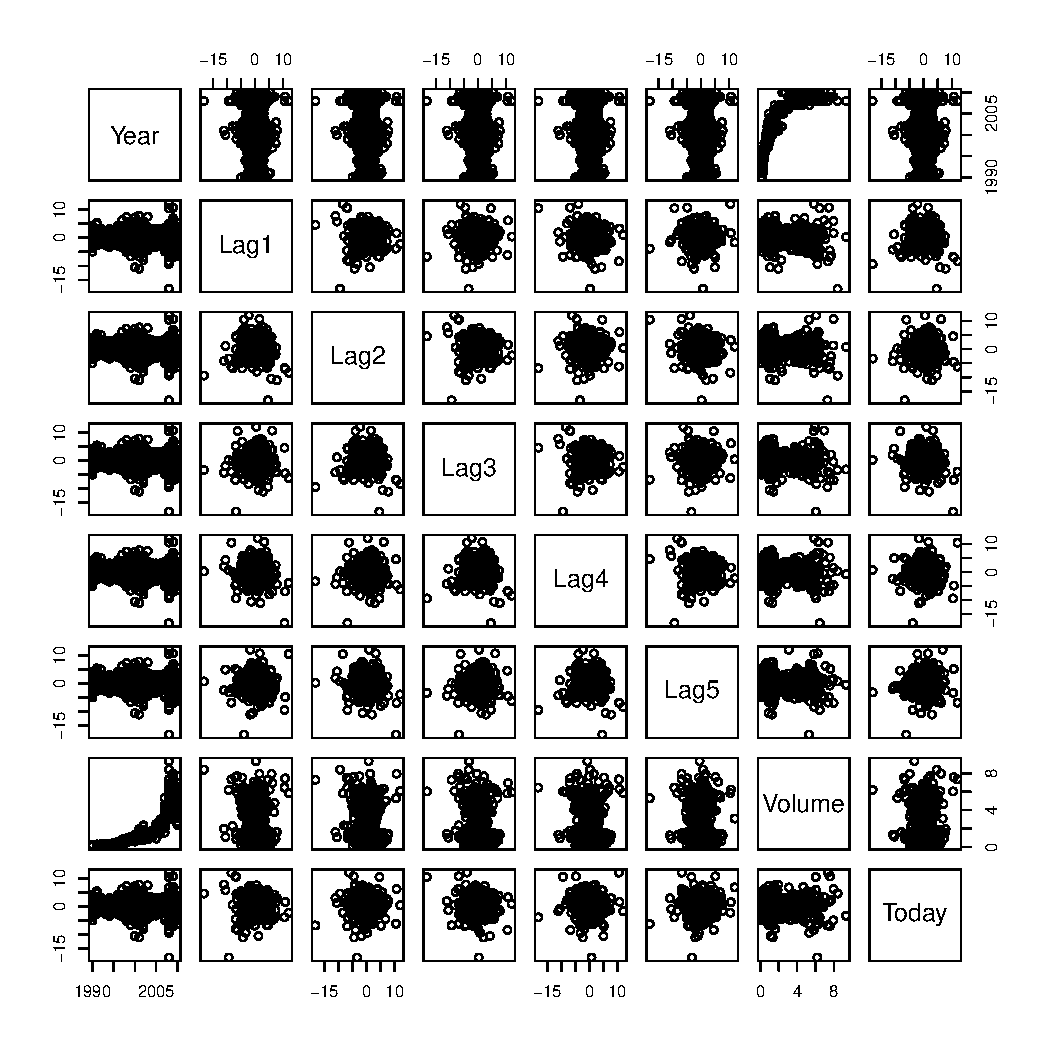
\includegraphics[width=\maxwidth]{figure/unnamed-chunk-2-1} 

\end{knitrout}
There are a few interesting places of correlation. Primarily, with Volume and Year. Other wise, it is observable that each of the Lags are clustered, but it is difficult to observe other relationships.

\item
\begin{knitrout}
\definecolor{shadecolor}{rgb}{0.969, 0.969, 0.969}\color{fgcolor}\begin{kframe}
\begin{alltt}
\hlstd{glm.fit}\hlkwb{=}\hlkwd{glm}\hlstd{(Direction}\hlopt{~}\hlstd{Lag1}\hlopt{+}\hlstd{Lag2}\hlopt{+}\hlstd{Lag3}\hlopt{+}\hlstd{Lag4}\hlopt{+}\hlstd{Lag5}\hlopt{+}\hlstd{Volume,}\hlkwc{data}\hlstd{=Weekly,} \hlkwc{family} \hlstd{= binomial)}
\hlkwd{summary}\hlstd{(glm.fit)}
\end{alltt}
\begin{verbatim}
## 
## Call:
## glm(formula = Direction ~ Lag1 + Lag2 + Lag3 + Lag4 + Lag5 + 
##     Volume, family = binomial, data = Weekly)
## 
## Deviance Residuals: 
##     Min       1Q   Median       3Q      Max  
## -1.6949  -1.2565   0.9913   1.0849   1.4579  
## 
## Coefficients:
##             Estimate Std. Error z value Pr(>|z|)   
## (Intercept)  0.26686    0.08593   3.106   0.0019 **
## Lag1        -0.04127    0.02641  -1.563   0.1181   
## Lag2         0.05844    0.02686   2.175   0.0296 * 
## Lag3        -0.01606    0.02666  -0.602   0.5469   
## Lag4        -0.02779    0.02646  -1.050   0.2937   
## Lag5        -0.01447    0.02638  -0.549   0.5833   
## Volume      -0.02274    0.03690  -0.616   0.5377   
## ---
## Signif. codes:  0 '***' 0.001 '**' 0.01 '*' 0.05 '.' 0.1 ' ' 1
## 
## (Dispersion parameter for binomial family taken to be 1)
## 
##     Null deviance: 1496.2  on 1088  degrees of freedom
## Residual deviance: 1486.4  on 1082  degrees of freedom
## AIC: 1500.4
## 
## Number of Fisher Scoring iterations: 4
\end{verbatim}
\begin{alltt}
\hlkwd{coef}\hlstd{(glm.fit)}
\end{alltt}
\begin{verbatim}
## (Intercept)        Lag1        Lag2        Lag3        Lag4        Lag5 
##  0.26686414 -0.04126894  0.05844168 -0.01606114 -0.02779021 -0.01447206 
##      Volume 
## -0.02274153
\end{verbatim}
\end{kframe}
\end{knitrout}

The only predictors which have significance are the intercept and Lag2. Lag2 is between $95\%$ and $99\%$ significant. The Intercept is $99\%$ and $99.9\%$.

\item
\begin{knitrout}
\definecolor{shadecolor}{rgb}{0.969, 0.969, 0.969}\color{fgcolor}\begin{kframe}
\begin{alltt}
\hlkwd{contrasts}\hlstd{(Direction)}
\end{alltt}
\begin{verbatim}
##      Up
## Down  0
## Up    1
\end{verbatim}
\begin{alltt}
\hlstd{glm.pred}\hlkwb{=}\hlkwd{rep}\hlstd{(}\hlstr{"Down"}\hlstd{,} \hlnum{1089}\hlstd{)}
\hlstd{glm.probs}\hlkwb{=}\hlkwd{predict}\hlstd{(glm.fit,}\hlkwc{type}\hlstd{=}\hlstr{"response"}\hlstd{)}
\hlstd{glm.probs[}\hlnum{1}\hlopt{:}\hlnum{10}\hlstd{]}
\end{alltt}
\begin{verbatim}
##         1         2         3         4         5         6         7 
## 0.6086249 0.6010314 0.5875699 0.4816416 0.6169013 0.5684190 0.5786097 
##         8         9        10 
## 0.5151972 0.5715200 0.5554287
\end{verbatim}
\begin{alltt}
\hlstd{glm.pred[glm.probs}\hlopt{>}\hlnum{0.5}\hlstd{]}\hlkwb{<-}\hlstr{"Up"}
\hlkwd{table}\hlstd{(glm.pred,Direction)}
\end{alltt}
\begin{verbatim}
##         Direction
## glm.pred Down  Up
##     Down   54  48
##     Up    430 557
\end{verbatim}
\begin{alltt}
\hlnum{557}\hlopt{/}\hlstd{(}\hlnum{557}\hlopt{+}\hlnum{430}\hlstd{)}
\end{alltt}
\begin{verbatim}
## [1] 0.5643364
\end{verbatim}
\begin{alltt}
\hlnum{430}\hlopt{/}\hlstd{(}\hlnum{557}\hlopt{+}\hlnum{430}\hlstd{)}
\end{alltt}
\begin{verbatim}
## [1] 0.4356636
\end{verbatim}
\begin{alltt}
\hlnum{48}\hlopt{/}\hlstd{(}\hlnum{48}\hlopt{+}\hlnum{54}\hlstd{)}
\end{alltt}
\begin{verbatim}
## [1] 0.4705882
\end{verbatim}
\end{kframe}
\end{knitrout}

The confusion matrix shows that on days when logistic regression predicts an increase in the market, it has a $56.4\%$ accuracy rate. The error rate is $43.6\%$ for predicting Up and is actually Down. The error rate is $47.1\%$ for predicting Down and is actually Up.

\item
\begin{knitrout}
\definecolor{shadecolor}{rgb}{0.969, 0.969, 0.969}\color{fgcolor}\begin{kframe}
\begin{alltt}
\hlstd{glm.fit2}\hlkwb{=}\hlkwd{glm}\hlstd{(Direction}\hlopt{~}\hlstd{Lag2,}\hlkwc{data}\hlstd{=Weekly,} \hlkwc{family} \hlstd{= binomial)}
\hlkwd{summary}\hlstd{(glm.fit2)}
\end{alltt}
\begin{verbatim}
## 
## Call:
## glm(formula = Direction ~ Lag2, family = binomial, data = Weekly)
## 
## Deviance Residuals: 
##    Min      1Q  Median      3Q     Max  
## -1.564  -1.267   1.008   1.086   1.386  
## 
## Coefficients:
##             Estimate Std. Error z value Pr(>|z|)    
## (Intercept)  0.21473    0.06123   3.507 0.000453 ***
## Lag2         0.06279    0.02636   2.382 0.017230 *  
## ---
## Signif. codes:  0 '***' 0.001 '**' 0.01 '*' 0.05 '.' 0.1 ' ' 1
## 
## (Dispersion parameter for binomial family taken to be 1)
## 
##     Null deviance: 1496.2  on 1088  degrees of freedom
## Residual deviance: 1490.4  on 1087  degrees of freedom
## AIC: 1494.4
## 
## Number of Fisher Scoring iterations: 4
\end{verbatim}
\begin{alltt}
\hlkwd{coef}\hlstd{(glm.fit2)}
\end{alltt}
\begin{verbatim}
## (Intercept)        Lag2 
##  0.21473151  0.06279058
\end{verbatim}
\begin{alltt}
\hlkwd{contrasts}\hlstd{(Direction)}
\end{alltt}
\begin{verbatim}
##      Up
## Down  0
## Up    1
\end{verbatim}
\begin{alltt}
\hlstd{glm.pred2}\hlkwb{=}\hlkwd{rep}\hlstd{(}\hlstr{"Down"}\hlstd{,} \hlnum{1089}\hlstd{)}
\hlstd{glm.probs2}\hlkwb{=}\hlkwd{predict}\hlstd{(glm.fit2,}\hlkwc{type}\hlstd{=}\hlstr{"response"}\hlstd{)}
\hlstd{glm.probs2[}\hlnum{1}\hlopt{:}\hlnum{10}\hlstd{]}
\end{alltt}
\begin{verbatim}
##         1         2         3         4         5         6         7 
## 0.5777243 0.5661029 0.5492840 0.5132426 0.6071571 0.5644982 0.5716776 
##         8         9        10 
## 0.5321015 0.5659641 0.5541137
\end{verbatim}
\begin{alltt}
\hlstd{glm.pred2[glm.probs2}\hlopt{>}\hlnum{0.5}\hlstd{]}\hlkwb{<-}\hlstr{"Up"}
\hlkwd{table}\hlstd{(glm.pred2,Direction)}
\end{alltt}
\begin{verbatim}
##          Direction
## glm.pred2 Down  Up
##      Down   33  26
##      Up    451 579
\end{verbatim}
\begin{alltt}
\hlnum{579}\hlopt{/}\hlstd{(}\hlnum{579}\hlopt{+}\hlnum{451}\hlstd{)}
\end{alltt}
\begin{verbatim}
## [1] 0.5621359
\end{verbatim}
\begin{alltt}
\hlnum{451}\hlopt{/}\hlstd{(}\hlnum{579}\hlopt{+}\hlnum{451}\hlstd{)}
\end{alltt}
\begin{verbatim}
## [1] 0.4378641
\end{verbatim}
\begin{alltt}
\hlnum{26}\hlopt{/}\hlstd{(}\hlnum{26}\hlopt{+}\hlnum{33}\hlstd{)}
\end{alltt}
\begin{verbatim}
## [1] 0.440678
\end{verbatim}
\end{kframe}
\end{knitrout}

The confusion matrix shows that on days when logistic regression predicts an increase in the market, it has a $56.2\%$ accuracy rate. The error rate is $43.8\%$ for predicting Up and is actually Down. The error rate is $44.1\%$ for predicting Down and is actually Up.
\end{enumerate}

\textbf{ANSWER FOR 11:} \\

\begin{enumerate}[(a)]

\item
\begin{knitrout}
\definecolor{shadecolor}{rgb}{0.969, 0.969, 0.969}\color{fgcolor}\begin{kframe}
\begin{alltt}
\hlcom{#install.packages("RCurl")}
\hlkwd{library}\hlstd{(RCurl)}
\end{alltt}


{\ttfamily\noindent\itshape\color{messagecolor}{\#\# Loading required package: bitops}}\begin{alltt}
\hlstd{dataset}\hlkwb{<-}\hlkwd{getURL}\hlstd{(}
    \hlstr{'https://raw.githubusercontent.com/Jwcrist/BusA/master/homeworks/Assignment%204/Auto.csv'}\hlstd{,}
    \hlkwc{ssl.verifypeer}\hlstd{=}\hlnum{0L}\hlstd{,} \hlkwc{followlocation}\hlstd{=}\hlnum{1L}\hlstd{)}
\hlstd{dataset1}\hlkwb{<-}\hlkwd{read.csv}\hlstd{(}\hlkwc{text}\hlstd{=dataset)}
\hlkwd{head}\hlstd{(dataset1,}\hlnum{3}\hlstd{)}
\end{alltt}
\begin{verbatim}
##   mpg cylinders displacement horsepower weight acceleration year origin
## 1  18         8          307        130   3504         12.0   70      1
## 2  15         8          350        165   3693         11.5   70      1
## 3  18         8          318        150   3436         11.0   70      1
##                        name mpg01
## 1 chevrolet chevelle malibu     0
## 2         buick skylark 320     0
## 3        plymouth satellite     0
\end{verbatim}
\end{kframe}
\end{knitrout}
As can be shown above we have created our binary data and a median column

\item
\begin{knitrout}
\definecolor{shadecolor}{rgb}{0.969, 0.969, 0.969}\color{fgcolor}\begin{kframe}
\begin{alltt}
\hlkwd{library}\hlstd{(dplyr)}
\end{alltt}


{\ttfamily\noindent\color{warningcolor}{\#\# Warning: package 'dplyr' was built under R version 3.1.2}}

{\ttfamily\noindent\itshape\color{messagecolor}{\#\# \\\#\# Attaching package: 'dplyr'\\\#\# \\\#\# The following object is masked from 'package:MASS':\\\#\# \\\#\#\ \ \ \  select\\\#\# \\\#\# The following object is masked from 'package:stats':\\\#\# \\\#\#\ \ \ \  filter\\\#\# \\\#\# The following objects are masked from 'package:base':\\\#\# \\\#\#\ \ \ \  intersect, setdiff, setequal, union}}\begin{alltt}
\hlstd{dataset2}\hlkwb{<-}\hlstd{dataset1} \hlopt

  \hlkwd{select}\hlstd{(mpg, cylinders, displacement,} \hlkwd{as.numeric}\hlstd{(horsepower), weight, acceleration, year, origin, mpg01)}
\hlkwd{str}\hlstd{(dataset2)}
\end{alltt}
\begin{verbatim}
## 'data.frame':	397 obs. of  9 variables:
##  $ mpg         : num  18 15 18 16 17 15 14 14 14 15 ...
##  $ cylinders   : int  8 8 8 8 8 8 8 8 8 8 ...
##  $ displacement: num  307 350 318 304 302 429 454 440 455 390 ...
##  $ horsepower  : Factor w/ 94 levels "?","100","102",..: 17 35 29 29 24 42 47 46 48 40 ...
##  $ weight      : int  3504 3693 3436 3433 3449 4341 4354 4312 4425 3850 ...
##  $ acceleration: num  12 11.5 11 12 10.5 10 9 8.5 10 8.5 ...
##  $ year        : int  70 70 70 70 70 70 70 70 70 70 ...
##  $ origin      : int  1 1 1 1 1 1 1 1 1 1 ...
##  $ mpg01       : int  0 0 0 0 0 0 0 0 0 0 ...
\end{verbatim}
\begin{alltt}
\hlkwd{cor}\hlstd{(dataset2)}
\end{alltt}


{\ttfamily\noindent\bfseries\color{errorcolor}{\#\# Error in cor(dataset2): 'x' must be numeric}}\begin{alltt}
\hlkwd{pairs}\hlstd{(dataset1)}
\end{alltt}
\end{kframe}
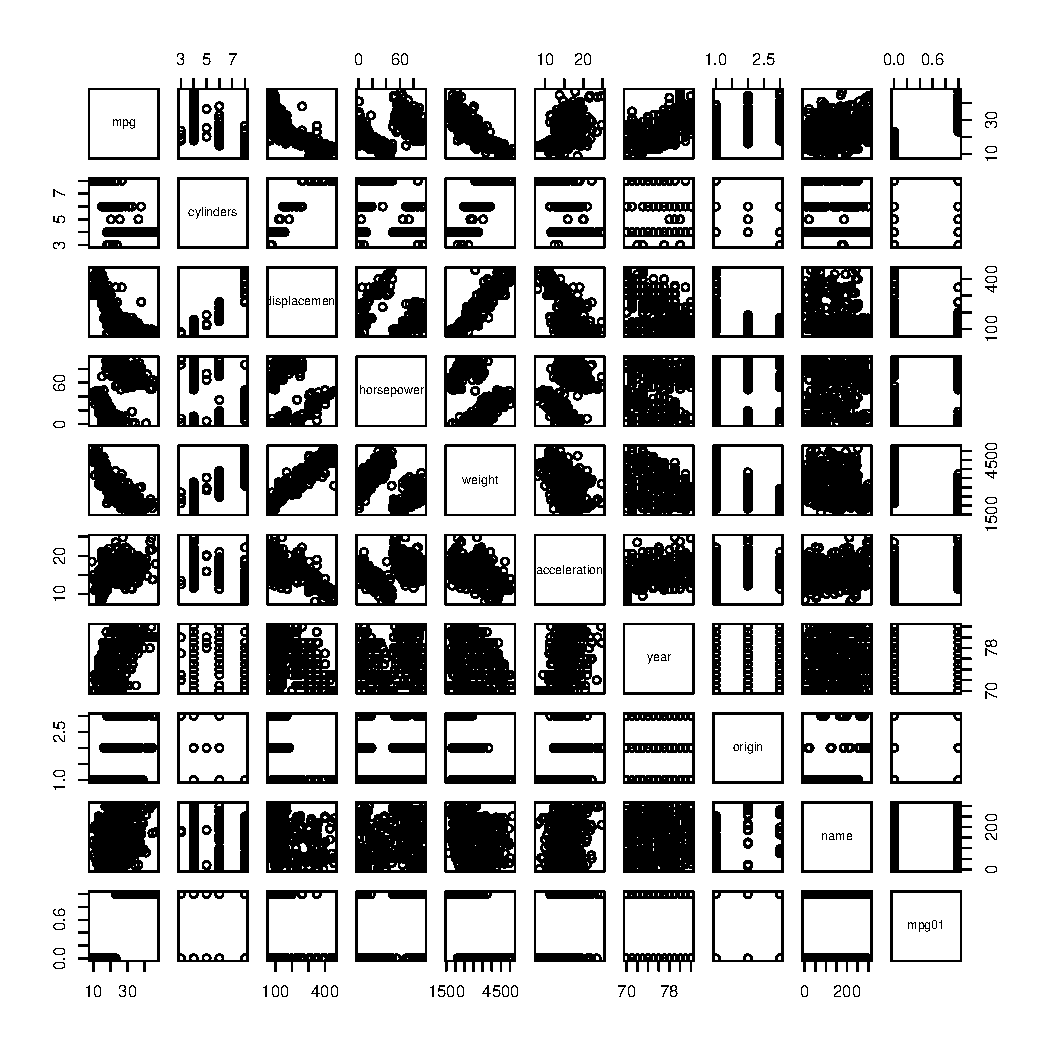
\includegraphics[width=\maxwidth]{figure/unnamed-chunk-7-1} 
\begin{kframe}\begin{alltt}
\hlkwd{library}\hlstd{(ggplot2)}
\hlkwd{ggplot}\hlstd{(dataset1,} \hlkwd{aes}\hlstd{(}\hlkwc{x}\hlstd{=}\hlkwd{factor}\hlstd{(mpg01),} \hlkwc{y}\hlstd{=mpg))}\hlopt{+}\hlkwd{geom_boxplot}\hlstd{()}
\end{alltt}
\end{kframe}
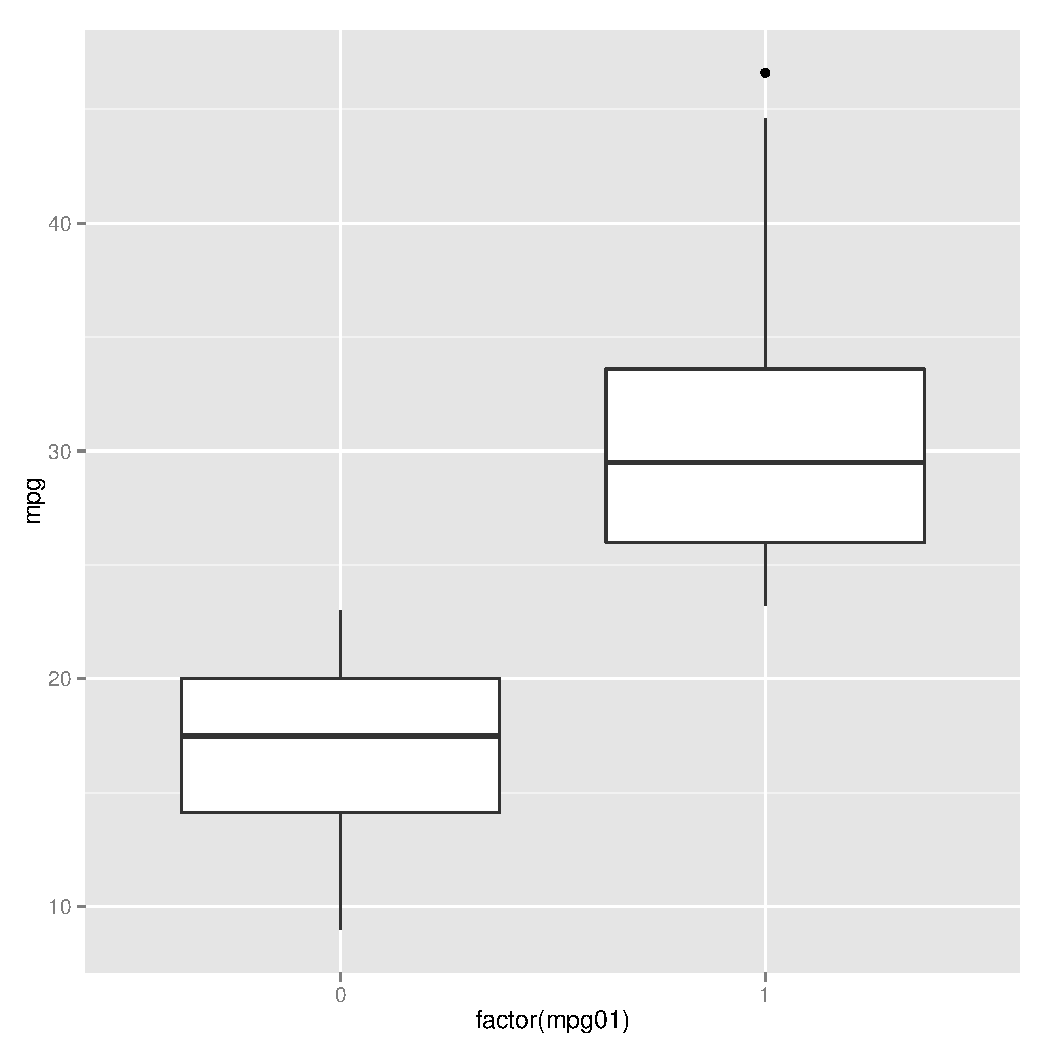
\includegraphics[width=\maxwidth]{figure/unnamed-chunk-7-2} 
\begin{kframe}\begin{alltt}
\hlkwd{ggplot}\hlstd{(dataset1,} \hlkwd{aes}\hlstd{(}\hlkwc{x}\hlstd{=}\hlkwd{factor}\hlstd{(mpg01),} \hlkwc{y}\hlstd{=cylinders))}\hlopt{+}\hlkwd{geom_boxplot}\hlstd{()}
\end{alltt}
\end{kframe}
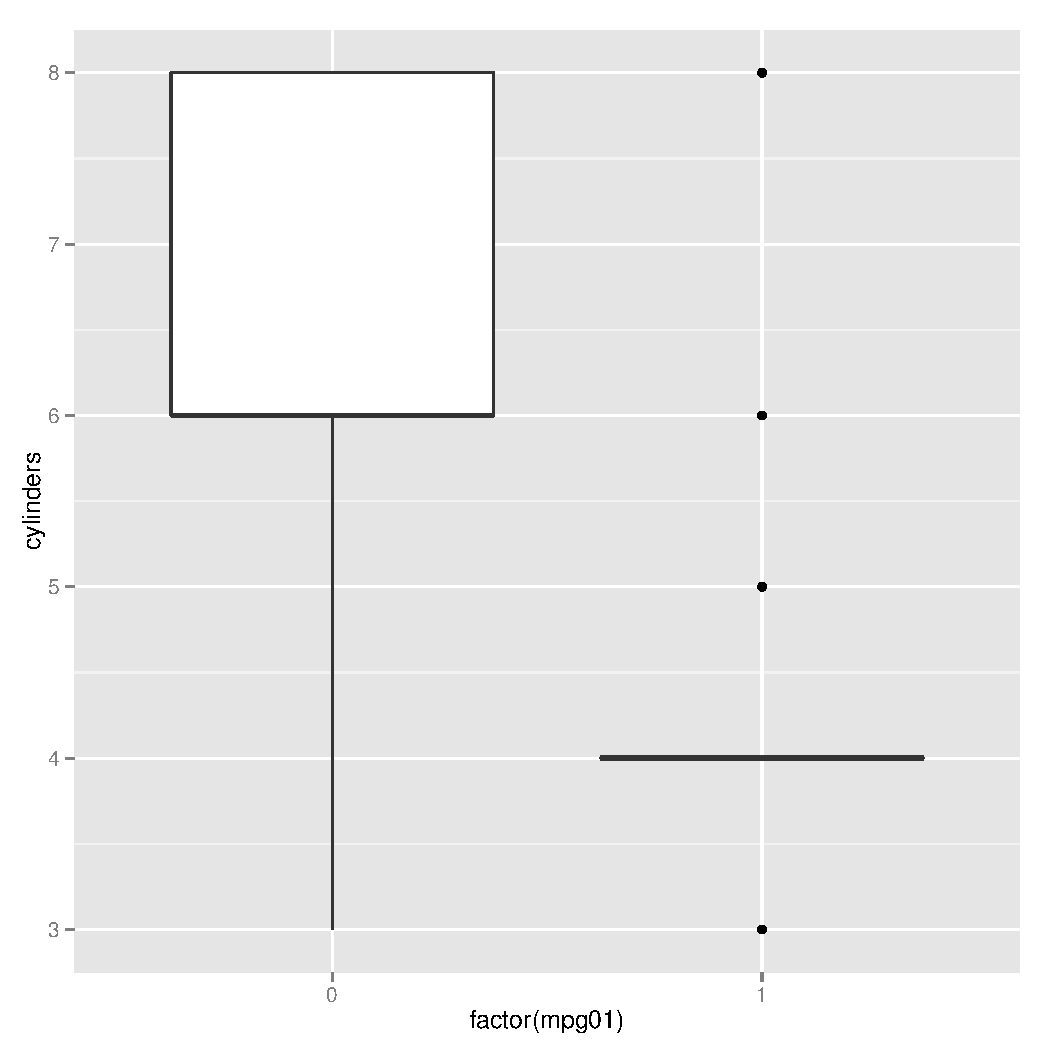
\includegraphics[width=\maxwidth]{figure/unnamed-chunk-7-3} 
\begin{kframe}\begin{alltt}
\hlkwd{ggplot}\hlstd{(dataset1,} \hlkwd{aes}\hlstd{(}\hlkwc{x}\hlstd{=}\hlkwd{factor}\hlstd{(mpg01),} \hlkwc{y}\hlstd{=displacement))}\hlopt{+}\hlkwd{geom_boxplot}\hlstd{()}
\end{alltt}
\end{kframe}
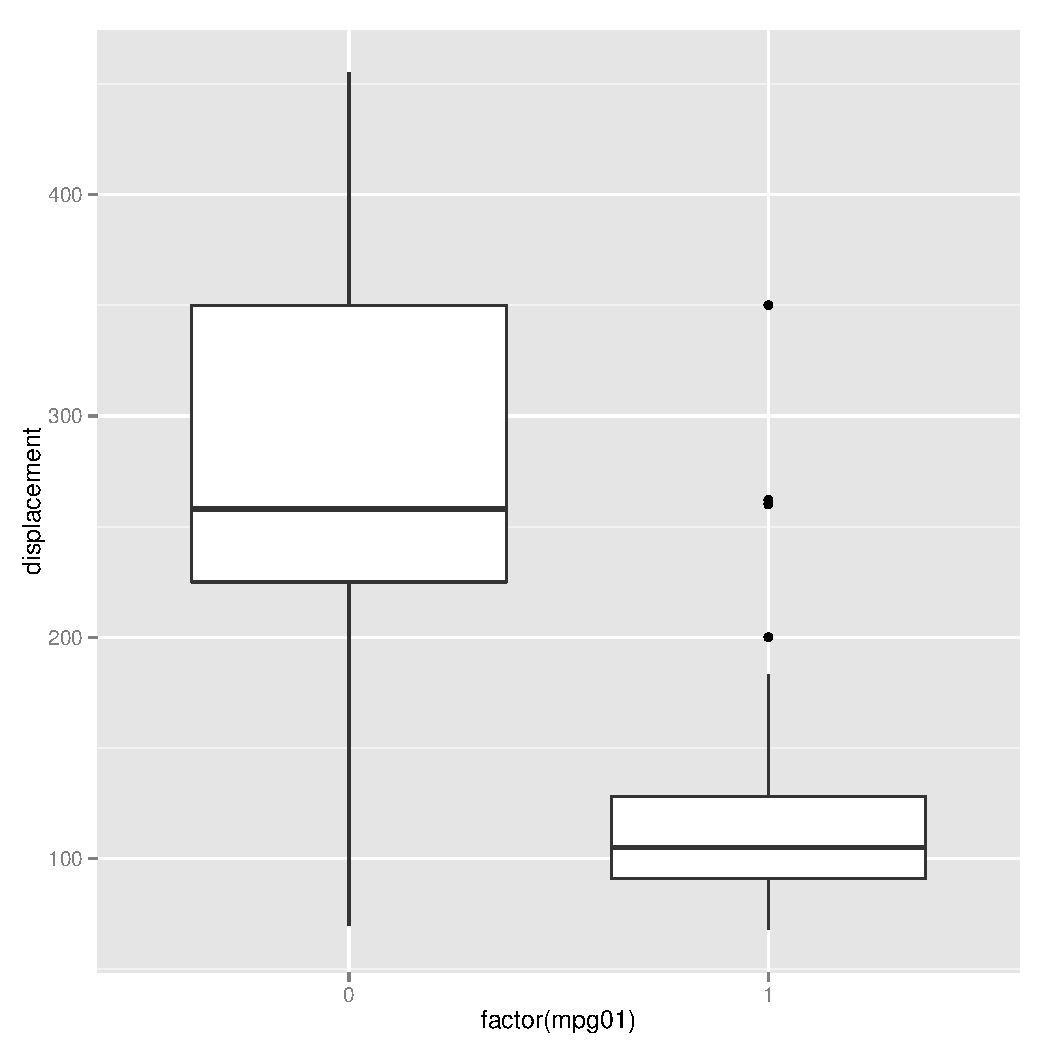
\includegraphics[width=\maxwidth]{figure/unnamed-chunk-7-4} 
\begin{kframe}\begin{alltt}
\hlkwd{ggplot}\hlstd{(dataset1,} \hlkwd{aes}\hlstd{(}\hlkwc{x}\hlstd{=}\hlkwd{factor}\hlstd{(mpg01),} \hlkwc{y}\hlstd{=weight))}\hlopt{+}\hlkwd{geom_boxplot}\hlstd{()}
\end{alltt}
\end{kframe}
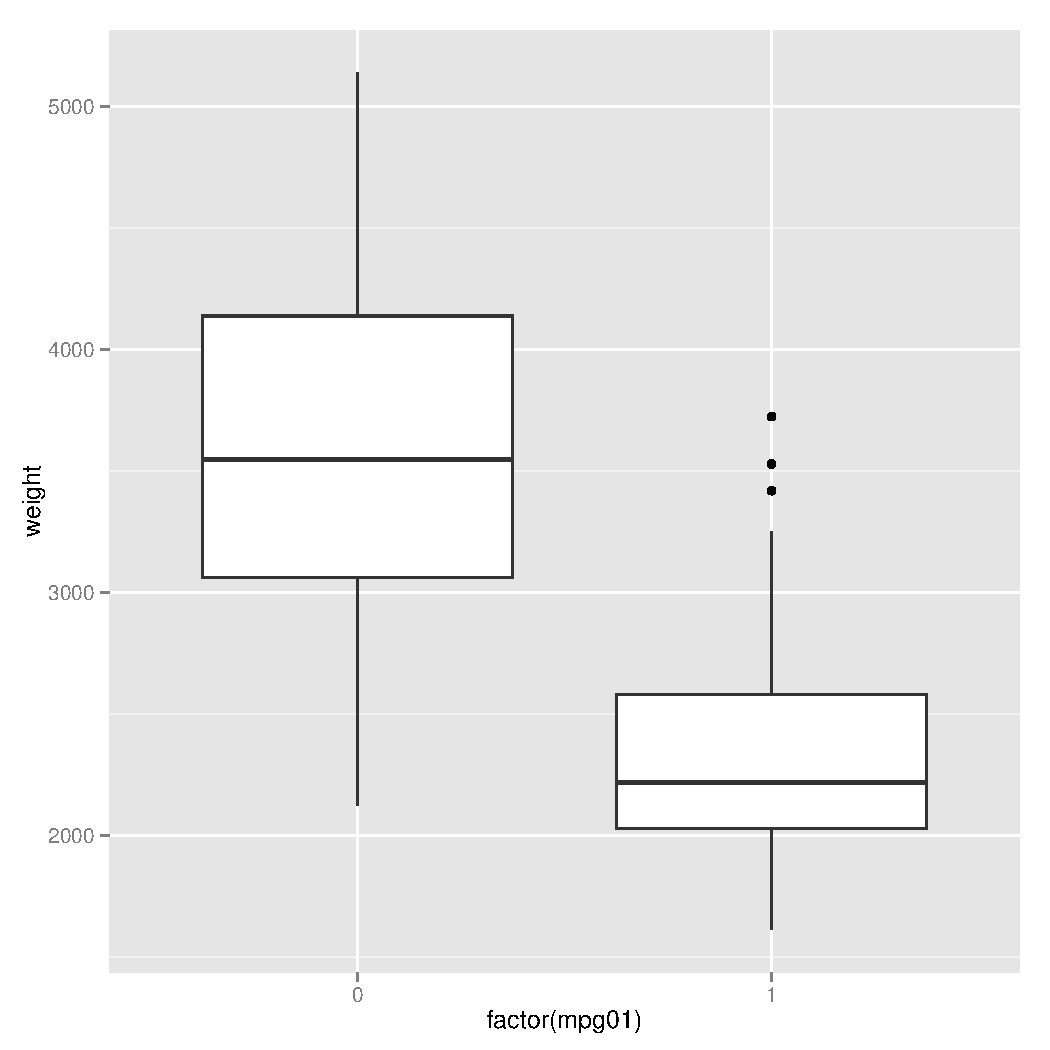
\includegraphics[width=\maxwidth]{figure/unnamed-chunk-7-5} 
\begin{kframe}\begin{alltt}
\hlkwd{ggplot}\hlstd{(dataset1,} \hlkwd{aes}\hlstd{(}\hlkwc{x}\hlstd{=}\hlkwd{factor}\hlstd{(mpg01),} \hlkwc{y}\hlstd{=acceleration))}\hlopt{+}\hlkwd{geom_boxplot}\hlstd{()}
\end{alltt}
\end{kframe}
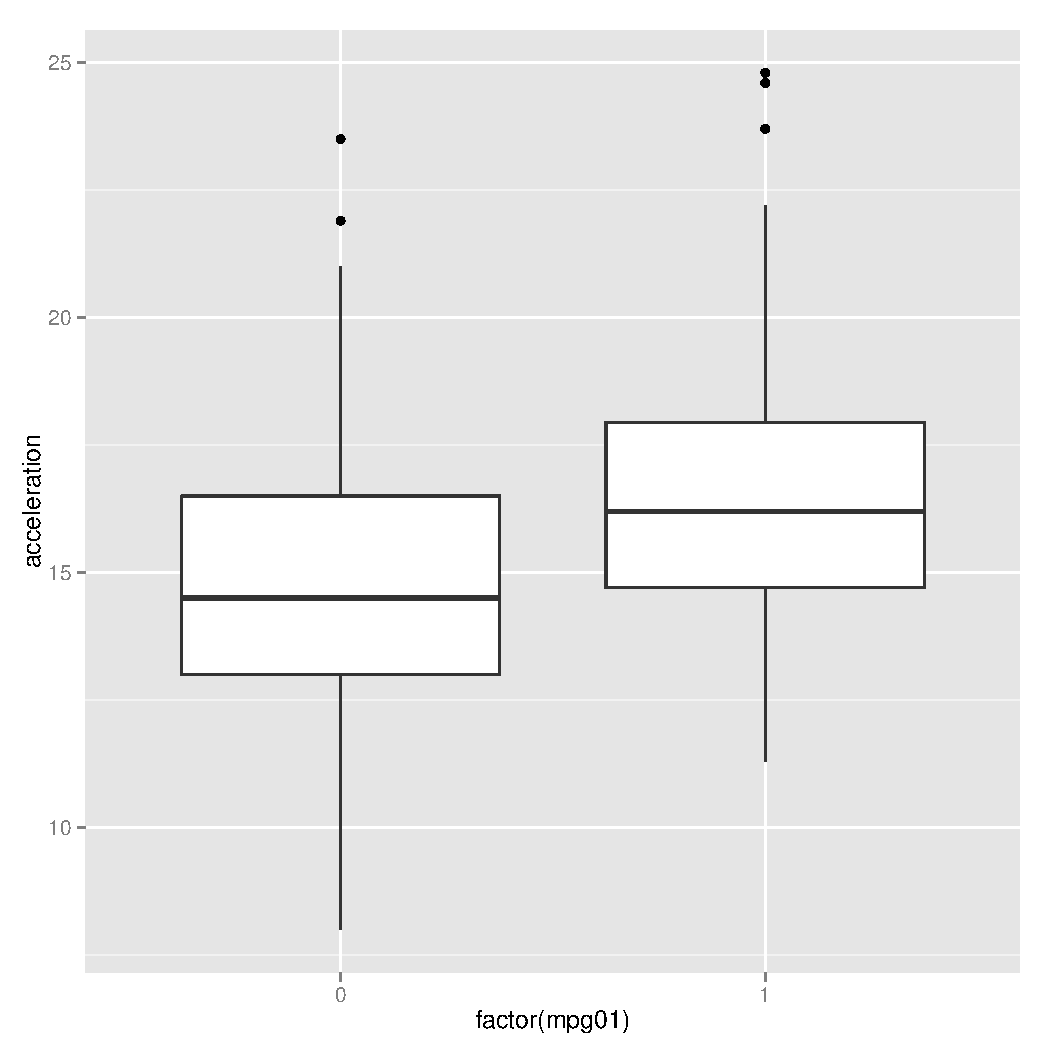
\includegraphics[width=\maxwidth]{figure/unnamed-chunk-7-6} 
\begin{kframe}\begin{alltt}
\hlkwd{ggplot}\hlstd{(dataset1,} \hlkwd{aes}\hlstd{(}\hlkwc{x}\hlstd{=}\hlkwd{factor}\hlstd{(mpg01),} \hlkwc{y}\hlstd{=year))}\hlopt{+}\hlkwd{geom_boxplot}\hlstd{()}
\end{alltt}
\end{kframe}
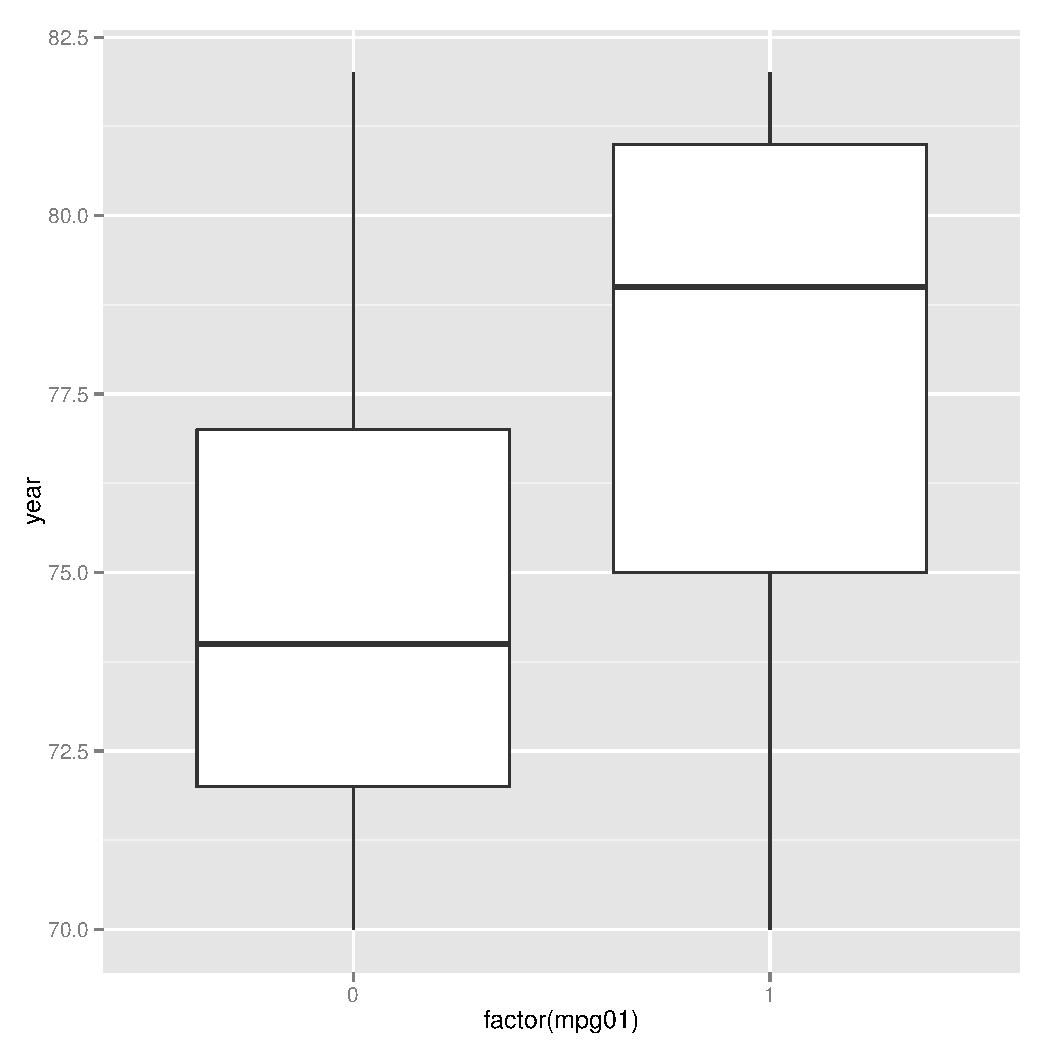
\includegraphics[width=\maxwidth]{figure/unnamed-chunk-7-7} 

\end{knitrout}

There is too many layers to observe anything of significance in horsepower. Acceleration and year may have be significantly different from eachother. All the other plots show that there is probable differences between our binary factors.
\item
\begin{knitrout}
\definecolor{shadecolor}{rgb}{0.969, 0.969, 0.969}\color{fgcolor}\begin{kframe}
\begin{alltt}
\hlkwd{tail}\hlstd{(dataset1)}
\end{alltt}
\begin{verbatim}
##     mpg cylinders displacement horsepower weight acceleration year origin
## 392  27         4          151         90   2950         17.3   82      1
## 393  27         4          140         86   2790         15.6   82      1
## 394  44         4           97         52   2130         24.6   82      2
## 395  32         4          135         84   2295         11.6   82      1
## 396  28         4          120         79   2625         18.6   82      1
## 397  31         4          119         82   2720         19.4   82      1
##                 name mpg01
## 392 chevrolet camaro     1
## 393  ford mustang gl     1
## 394        vw pickup     1
## 395    dodge rampage     1
## 396      ford ranger     1
## 397       chevy s-10     1
\end{verbatim}
\begin{alltt}
\hlstd{trainingdata}\hlkwb{<-}\hlstd{dataset1[}\hlnum{1}\hlopt{:}\hlnum{318}\hlstd{,]}
\hlstd{testdata}\hlkwb{<-}\hlstd{dataset1[}\hlnum{79}\hlstd{,]}
\end{alltt}
\end{kframe}
\end{knitrout}
A $80\%$ training data set was choosen to be used inorder to prove against our test data.

\item
Do Not Do
\item
Do Not Do
\item
\begin{knitrout}
\definecolor{shadecolor}{rgb}{0.969, 0.969, 0.969}\color{fgcolor}\begin{kframe}
\begin{alltt}
\hlstd{glm.fit3}\hlkwb{=}\hlkwd{glm}\hlstd{(mpg01}\hlopt{~}\hlstd{Lag2,}\hlkwc{data}\hlstd{=Weekly,} \hlkwc{family} \hlstd{= binomial)}
\end{alltt}


{\ttfamily\noindent\bfseries\color{errorcolor}{\#\# Error in eval(expr, envir, enclos): object 'mpg01' not found}}\begin{alltt}
\hlkwd{summary}\hlstd{(glm.fit2)}
\end{alltt}
\begin{verbatim}
## 
## Call:
## glm(formula = Direction ~ Lag2, family = binomial, data = Weekly)
## 
## Deviance Residuals: 
##    Min      1Q  Median      3Q     Max  
## -1.564  -1.267   1.008   1.086   1.386  
## 
## Coefficients:
##             Estimate Std. Error z value Pr(>|z|)    
## (Intercept)  0.21473    0.06123   3.507 0.000453 ***
## Lag2         0.06279    0.02636   2.382 0.017230 *  
## ---
## Signif. codes:  0 '***' 0.001 '**' 0.01 '*' 0.05 '.' 0.1 ' ' 1
## 
## (Dispersion parameter for binomial family taken to be 1)
## 
##     Null deviance: 1496.2  on 1088  degrees of freedom
## Residual deviance: 1490.4  on 1087  degrees of freedom
## AIC: 1494.4
## 
## Number of Fisher Scoring iterations: 4
\end{verbatim}
\begin{alltt}
\hlkwd{coef}\hlstd{(glm.fit2)}
\end{alltt}
\begin{verbatim}
## (Intercept)        Lag2 
##  0.21473151  0.06279058
\end{verbatim}
\begin{alltt}
\hlkwd{contrasts}\hlstd{(Direction)}
\end{alltt}
\begin{verbatim}
##      Up
## Down  0
## Up    1
\end{verbatim}
\begin{alltt}
\hlstd{glm.pred2}\hlkwb{=}\hlkwd{rep}\hlstd{(}\hlstr{"Down"}\hlstd{,} \hlnum{1089}\hlstd{)}
\hlstd{glm.probs2}\hlkwb{=}\hlkwd{predict}\hlstd{(glm.fit2,}\hlkwc{type}\hlstd{=}\hlstr{"response"}\hlstd{)}
\hlstd{glm.probs2[}\hlnum{1}\hlopt{:}\hlnum{10}\hlstd{]}
\end{alltt}
\begin{verbatim}
##         1         2         3         4         5         6         7 
## 0.5777243 0.5661029 0.5492840 0.5132426 0.6071571 0.5644982 0.5716776 
##         8         9        10 
## 0.5321015 0.5659641 0.5541137
\end{verbatim}
\begin{alltt}
\hlstd{glm.pred2[glm.probs2}\hlopt{>}\hlnum{0.5}\hlstd{]}\hlkwb{<-}\hlstr{"Up"}
\hlkwd{table}\hlstd{(glm.pred2,Direction)}
\end{alltt}
\begin{verbatim}
##          Direction
## glm.pred2 Down  Up
##      Down   33  26
##      Up    451 579
\end{verbatim}
\end{kframe}
\end{knitrout}
\end{enumerate}

\end{document}
